\begin{tframe}{Introduction}

\textbf{Objective}: the creation of a procedure, based on the work of [1], thanks to which build a large dataset of images of faces that can be used in the training process of a \textbf{CNN}.

\begin{figure}[h]
\begin{center}
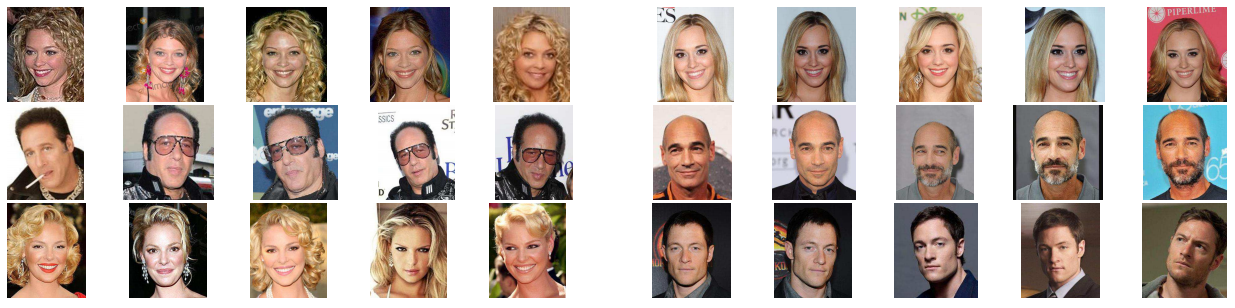
\includegraphics[width=0.9\textwidth]{images/image12.png}
\end{center}
\end{figure}

This procedure takes advantage of the modern \textbf{search engines}, and, at the same time, has the objective of decreasing at a minimum the cost in terms of human time necessary to the acquisition and annotations of the images of the dataset.

\end{tframe}

\begin{tframe}{Introduction}

The proposed method is divided in phases, as follows:

\begin{itemize}
\item A \textbf{dataset creation} phases, by exploiting modern search engines.
\item Detect the faces inside the downloaded images thanks to a \textbf{face detector}.
\item A \textbf{duplicate removal} phase, thanks to which duplicate images are removed.
\item A \textbf{classification} phase, to determine if the faces are correctly associated to an identity.
\item A \textbf{visual validation} phase, done by a user with the help of a web application.
\end{itemize}

\begin{figure}[plain]
    \hspace*{-9mm}
    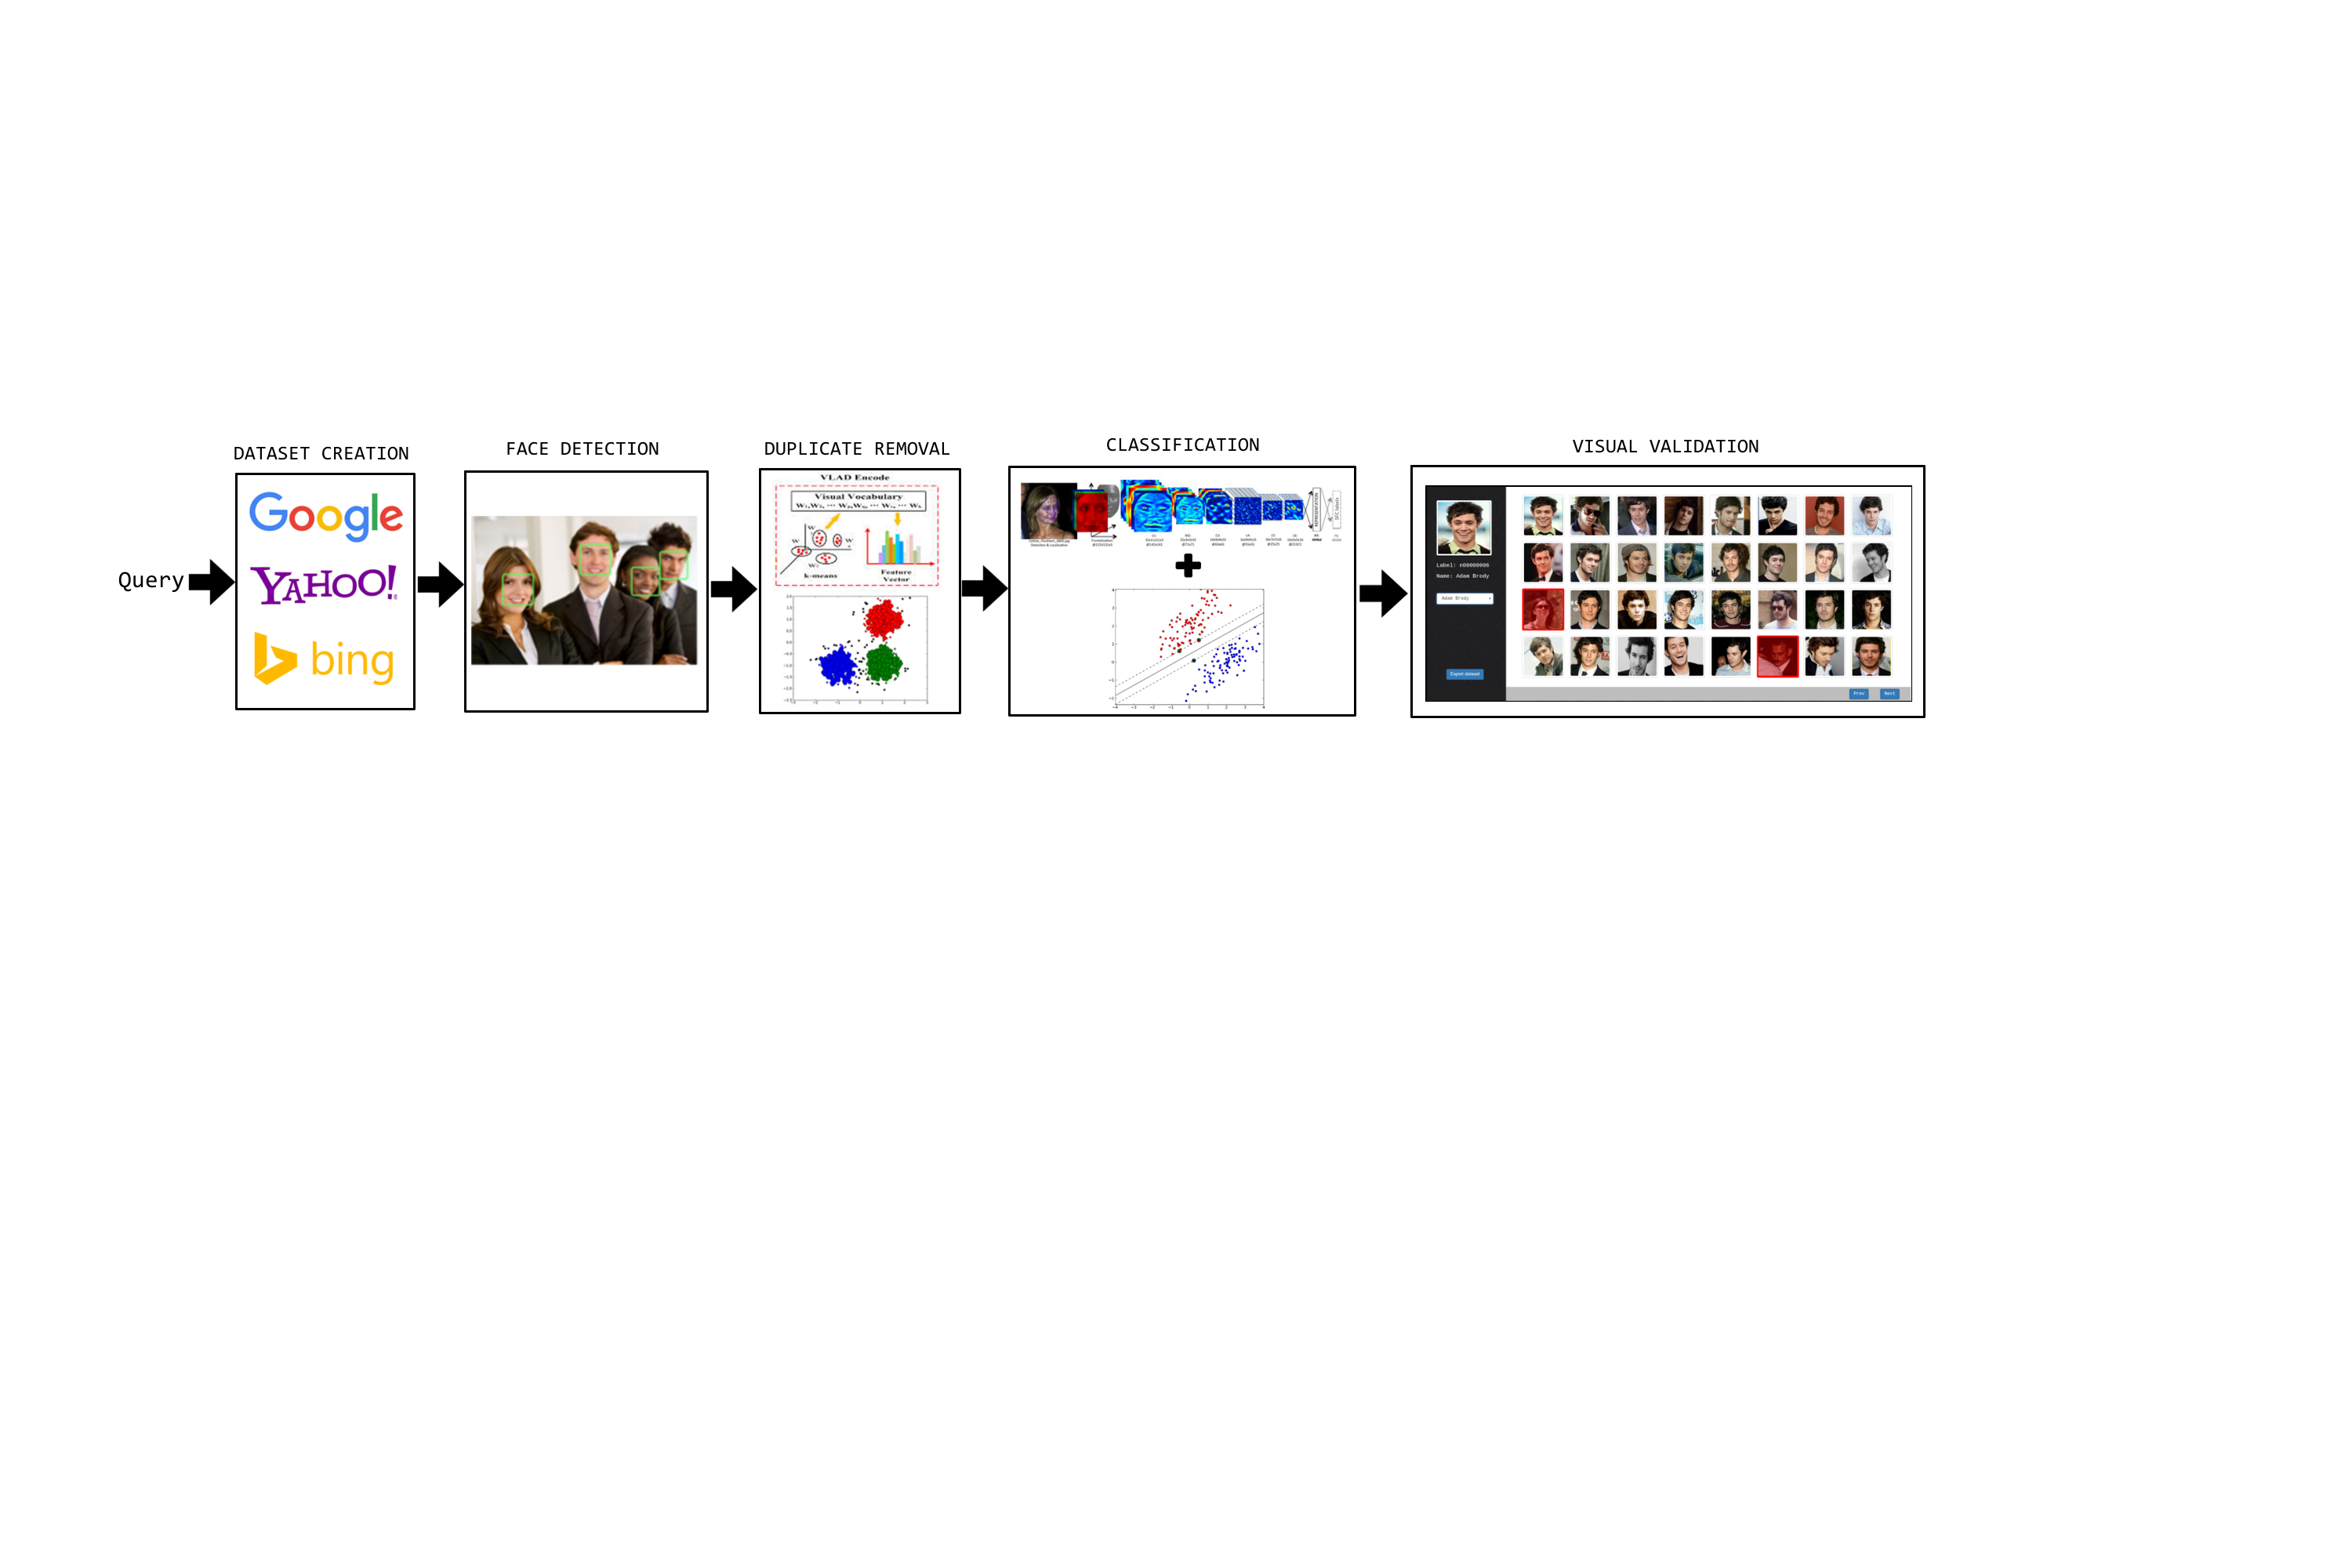
\includegraphics[width=\paperwidth]{images/pipeline2.png}
\end{figure} 


\end{tframe}